\section{Marco de Referencia}
\subsection{Marco Teórico}

\subsubsection{Sonido.} El sonido se puede definir de formas muy diversas. De todas ellas, las más habituales 
son las siguientes:

\begin{itemize}
    \item 
    Vibración mecánica que se propaga a través de un medio (habitualmente el aire), y que es 
    capaz de producir una sensación auditiva. 
    \item
    Sensación auditiva producida por una vibración de carácter mecánico que se propaga a través de un medio \cite{Isbert1998}.   
\end{itemize}

\subsubsection{Generación y propagación del sonido.} El elemento generador del sonido se denomina 
fuente sonora (tambor, cuerda de un violín, cuerdas vocales, etc.). La generación del sonido 
tiene lugar cuando dicha fuente entra en vibración. Dicha vibración es transmitida a las 
partículas de aire adyacentes a la misma que, a su vez, la transmiten a nuevas partículas 
contiguas.

Las partículas no se desplazan con la perturbación, sino que simplemente oscilan alrededor 
de su posición de equilibrio. La manera en que la perturbación se traslada de un lugar a otro 
se denomina propagación de la onda sonora. La oscilación de las partículas tiene lugar en la 
misma dirección que la de propagación de la onda \cite{Isbert1998}.

Ahora nos preguntamos qué tan rápido se aleja la onda de la fuente. La respuesta es que el 
sonido se propaga con una velocidad c que en el aire a 23ºC vale
\begin{equation}
c = 345 \quad\text{m/s,}
\end{equation}
o bien 
\begin{equation}
c = 1242 \quad\text{km/h,}
\end{equation}
Esta velocidad varía algo con la temperatura (un \textbf{0.17} $\% / ^{\circ} C$),  por eso en diversos textos pueden encontrarse valores ligeramente diferentes \cite{Miyara2004}. 

\subsubsection{Presión sonora.} La manera más habitual de expresar cuantitativamente la magnitud de un campo sonoro es mediante la presión sonora, o fuerza que ejercen las partículas de aire por unidad de superficie \cite{Isbert1998}.

Si nos ubicamos en una posición fija, veremos que la presión atmosférica aumenta y disminuye periódicamente, conforme pasan por el lugar las sucesivas perturbaciones. Dado que nos referiremos bastante seguido a valores de presión, conviene aclarar que la unidad adoptada internacionalmente para la presión es el Pascal, abreviada Pa. Expresada en esta unidad, la presión atmosférica es del orden de 100,000 Pa. Los aumentos y las disminuciones de presión debidas a las ondas sonoras son realmente muy pequeños comparados con este valor de presión atmosférica. Los sonidos más intensos que se perciben como tales implican un aumento de unos 20 Pa. La presión sonora es lo que se debe agregar a la presión atmosférica en reposo para obtener el valor real de presión atmosférica. Las presiones sonoras audibles varían entre 0,00002 Pa y 20 Pa. El valor más pequeño, también expresado como 20 µPa se denomina umbral auditivo \cite{Miyara2004}. 

\subsubsection{Tren de pulsos.} Es una variante de la onda cuadrada en el cual el tiempo de permanencia en cada uno de los dos niveles no es el mismo. Se suele especificar un porcentaje que corresponde a la porción del periodo en el nivel alto \cite{Miyara2004}.

\subsubsection{Acústica.} Es la disciplina que se ocupa para estudiar el sonido en sus diversos aspectos. Se puede dividir en una gran cantidad de sub disciplinas \cite{Miyara2004}, algunas de las cuales son la acústica física, la psico acústica, la acústica musical y en la cual nos centraremos nosotros, es la acústica arquitectónica. 

\subsubsection{Acústica Arquitectónica.} Estudia los fenómenos vinculados con una propagación adecuada, fiel y funcional del sonido en un recinto. Las habitaciones o salas dedicadas a una aplicación determinada deben tener cualidades acústicas adecuadas para dicha aplicación. Por cualidades acústicas de un recinto entendemos una serie de propiedades relacionadas con el comportamiento del sonido en el recinto, entre las cuales se encuentran las reflexiones tempranas, la reverberación, la existencia o no de ecos y resonancias, la cobertura sonora de las fuentes, etc. \cite{Miyara2004}.

\subsubsection{Ecos.} El fenómeno más sencillo que tiene lugar en un ambiente con superficies reflectoras del sonido es el eco, consistente en una única reflexión que retorna al punto donde se encuentra la fuente unos 100 ms (o más) después de emitido el sonido. Se produce después de un tiempo t relacionado con la distancia d a la superficie más próxima por la expresión

\begin{equation}
t = \frac{2d}{c},
\end{equation}

donde c es la velocidad del sonido. El factor 2 se debe a que el sonido recorre de ida y de vuelta la distancia entre la fuente sonora y la superficie \cite{Miyara2004}.

\subsubsection{Reflexiones tempranas.} Cuando la fuente sonora está rodeada por varias superficies (piso, paredes, techo) un oyente recibirá el sonido directo, y además el sonido reflejado en cada pared. Las primeras reflexiones recibidas, que se encuentran bastante separadas en el tiempo, se denominan reflexiones tempranas \cite{Miyara2004}.

\subsubsection{Absorción sonora.} Las superficies de un recinto reflejan solo parcialmente el sonido que incide sobre ellas; el resto es absorbido. Según el tipo de material o recubrimiento de una pared, ésta podrá absorber más o menos el sonido, lo cual lleva a definir el coeficiente de absorción sonora, abreviado con la letra griega $\alpha$ (alfa), como el cociente entre la energía absorbida y la energía incidente \cite{Miyara2004}:

\begin{equation}
a = \frac{E_{absorbida}}{E_{incidente}}
\end{equation}

El coeficiente de absorción tiene una gran importancia para el comportamiento acústico de un ambiente, y por esa razón se han medido y tabulado los coeficientes de absorción para varios materiales y objetos \cite{Miyara2004}.

%----------------------Tabla 2----------------------

\begin{center}
\footnotesize
    \begin{longtable}[!htb]{| m{22em} | m{2.5em} | m{2.5em} | m{2.5em} | m{2.5em} | m{2.5em} |m{2.5em} |}
    \hline
    \multirow{2}{*}{\textbf{Materiales}} & \multicolumn{6}{c|}{\textbf{Coeficiente de absorción $\alpha$ a la frecuencia}}\\
    \cline{2-7}
    & \textbf{125} & \textbf{250} & \textbf{500} & \textbf{1000} & \textbf{2000} & \textbf{4000} \\
    \hline
    Hormig\'on sin pintar & 0.01 & 0.01 & 0.02 & 0.02 & 0.04 & 0.04\\
    \hline
    Hormig\'on pintado & 0.01 & 0.01 & 0.01 & 0.02 & 0.02 & 0.02\\
    \hline
    Ladrillo visto sin pintar & 0.02 & 0.02 & 0.03 & 0.04 & 0.05 & 0.05\\
    \hline
    Ladrillo visto pintado & 0.01 & 0.01 & 0.02 & 0.02 & 0.02 & 0.02\\
    \hline
    Revoque de cal y arena & 0.04 & 0.05 & 0.06 & 0.08 & 0.04 & 0.06\\
    \hline
    Placa de yeso (Durlock) 12mm a 10cm & 0.29 & 0.10 & 0.05 & 0.04 & 0.07 & 0.09\\
    \hline
    Yeso sobre metal desplegado & 0.04 & 0.04 & 0.04 & 0.06 & 0.06 & 0.03\\
    \hline
    M\'armol o azulejo & 0.01 & 0.01 & 0.01 & 0.01 & 0.02 & 0.02\\
    \hline
    Madera en paneles (a 5cm de la pared) & 0.30 & 0.25 & 0.20 & 0.17 & 0.15 & 0.10\\
    \hline
    Madera aglomerada en panel & 0.47 & 0.52 & 0.50 & 0.55 & 0.58 & 0.63\\
    \hline
    Parquet & 0.04 & 0.04 & 0.07 & 0.06 & 0.06 & 0.07\\
    \hline
    Parquet sobre asfalto & 0.05 & 0.03 & 0.06 & 0.09 & 0.10 & 0.22\\
    \hline
    Parquet sobre listones & 0.20 & 0.15 & 0.12 & 0.10 & 0.10 & 0.07\\
    \hline
    Alfombra de goma 0.5cm & 0.04 & 0.04 & 0.08 & 0.12 & 0.03 & 0.10\\
    \hline
    Alfombra de lana 1.2$kg/m^2$ & 0.10 & 0.16 & 0.11 & 0.30 & 0.50 & 0.47\\
    \hline
    Alfombra de lana 2.3$kg/m^2$ & 0.17 & 0.18 & 0.21 & 0.50 & 0.63 & 0.83\\
    \hline 
    Cortina 338$g/m^2$ & 0.03 & 0.04 & 0.11 & 0.14 & 0.24 & 0.35\\
    \hline
    Cortina 338$g/m^2$ fruncida al 50\% & 0.07 & 0.31 & 0.49 & 0.75 & 0.70 & 0.60\\
    \hline
    Espuma de poliuretano (Fonac) 35mm & 0.11 & 0.14 & 0.36 & 0.82 & 0.90 & 0.97\\
    \hline
    Espuma de poliuretano (Fonac) 50mm & 0.15 & 0.25 & 0.50 & 0.94 & 0.92 & 0.99\\
    \hline
    Espuma de poliuretano (Fonac) 75mm & 0.17 & 0.44 & 0.99 & 1.03 & 1.00 & 1.03\\
    \hline
    Espuma de poliuretano (Sonex) 35mm & 0.06 & 0.20 & 0.45 & 0.71 & 0.95 & 0.89\\
    \hline
    Espuma de poliuretano (Sonex) 50mm & 0.07 & 0.32 & 0.72 & 0.88 & 0.97 & 1.01\\
    \hline
    Espuma de poliuretano (Sonex) 75mm & 0.13 & 0.53 & 0.90 & 1.07 & 1.07 & 1.00\\
    \hline
    Lana de vidrio (fieltro 14$kg/m^3$) 25mm & 0.15 & 0.25 & 0.40 & 0.50 & 0.65 & 0.70\\
    \hline
    Lana de vidrio (fieltro 14$kg/m^3$) 50mm & 0.25 & 0.45 & 0.70 & 0.80 & 0.85 & 0.85\\
    \hline
    Lana de vidrio (panel 14$kg/m^3$) 25mm & 0.20 & 0.40 & 0.80 & 0.90 & 1.00 & 1.00\\
    \hline
    Lana de vidrio (panel 14$kg/m^3$) 50mm & 0.30 & 0.75 & 1.00 & 1.00 & 1.00 & 1.00\\
    \hline
    Ventana abierta & 1.00 & 1.00 & 1.00 & 1.00 & 1.00 & 1.00\\
    \hline
    Vidrio & 0.03 & 0.02 & 0.02 & 0.01 & 0.07 & 0.04\\
    \hline
    Panel cielorraso Spanacustic (Manville) 19mm & - & 0.80 & 0.71 & 0.86 & 0.68 & -\\
    \hline
    Panel cielorraso Acustidom (Manville) 4mm & - & 0.72 & 0.61 & 0.68 & 0.79 & -\\
    \hline
    Panel cielorraso Prismatic (Manville) 19mm & - & 0.70 & 0.61 & 0.70 & 0.78 & -\\
    \hline
    Panel cielorraso Profil (Manville) 19mm & - & 0.72 & 0.62 & 0.69 & 0.78 & -\\
    \hline
    Panel cielorraso fisurado Auratone (USG) $5/8"$ & 0.34 & 0.36 & 0.71 & 0.85 & 0.68 & 0.64\\
    \hline
    Panel cielorraso fisurado Cortega (AWI) $5/8"$ & 0.31 & 0.32 & 0.51 & 0.72 & 0.74 & 0.77\\
    \hline
    Asiento de madera (0.8 $m^2/asiento$) & 0.01 & 0.02 & 0.03 & 0.04 & 0.06 & 0.08\\
    \hline
    Asiento tapizado grueso (0.8 $m^2/asiento$) & 0.44 & 0.44 & 0.44 & 0.44 & 0.44 & 0.44\\
    \hline
    Personas en asiento de madera (0.8 $m^2/persona$) & 0.34 & 0.39 & 0.44 & 0.54 & 0.56 & 0.56\\
    \hline
    Personas en asiento tapizado (0.8 $m^2/persona$) & 0.53 & 0.51 & 0.51 & 0.56 & 0.56 & 0.59\\
    \hline
    Personas de pie (0.8 $m^2/persona$) & 0.25 & 0.44 & 0.59 & 0.56 & 0.62 & 0.50\\
    \hline
    \caption{Coeficientes de absorción de diversos materiales en función de la frecuencia (según varias fuentes) \cite{Miyara2004}.}
    \label{tab:CoefMateriales}
    \end{longtable}
\end{center}
%----------------------Tabla 2----------------------

En la tabla 2 se dan los valores de $\alpha$ para varios materiales típicos de construcción, objetos y personas. Se proporcionan para varias frecuencias, ya que $\alpha$ depende bastante de la frecuencia \cite{Miyara2004}.
%tabla 2. Coficientes de absorcion.

\subsubsection{Tiempos de reverberación.} Después del periodo de las reflexiones tempranas, comienzan a aparecer las reflexiones de las reflexiones, y las reflexiones de las reflexiones de las reflexiones, y así sucesivamente, dando origen a una situación muy compleja en la cual las reflexiones se densifican cada vez más. Esta permanencia del sonido aún después de interrumpida la fuente se denomina reverberación. Para medir cuánto demora este proceso de extinción del sonido se introduce el concepto de tiempo de reverberación, T, técnicamente definido como el tiempo que demora el sonido en bajar 60 dB por debajo de su nivel inicial \cite{Miyara2004}.
\\
La propiedad anterior se puede expresar por medio de una fórmula, denominada fórmula de Sabine, en honor al físico norteamericano que la obtuvo a principios de este siglo. Según dicha fórmula el tiempo de reverberación T puede calcularse como:
\begin{equation}
T = 0.161\frac{V}{\alpha S}
\end{equation}
donde V es el volumen de la habitación en $m^3$, S es el área de su superficie interior total en $m^2$, y $\alpha$ es el coeficiente de absorción sonora [16].

\subsubsection{Tiempos de reverberación óptimo.} Varias investigaciones realizadas evaluando las acústicas de las mejores salas del mundo (según la opinión de las audiencias o usuarios y de expertos) han revelado que para cada finalidad existe un tiempo de reverberación óptimo, que aumenta al aumentar el volumen en $m^3$ de la sala.

En la ilustración 1 se muestra el resultado de uno de estos estudios. Debe aclararse que no hay coincidencia entre los resultados presentados por diversos investigadores, aunque cualitativamente son similares.

%Ilustracion 1 
\begin{figure}[!htb]
    \centering
    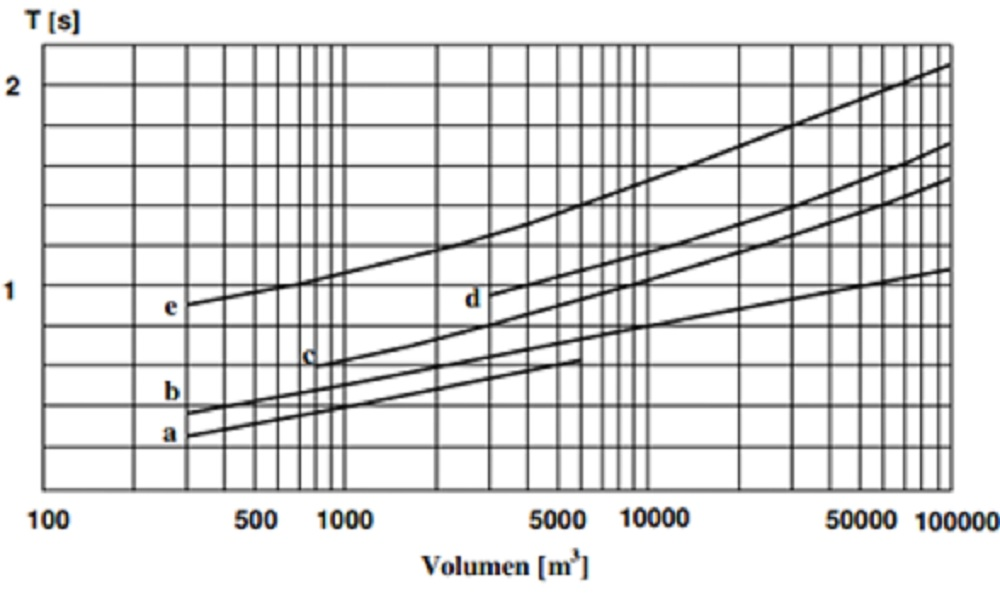
\includegraphics[width=0.7\textwidth]{imagenes/1.jpg}
    \caption{\footnotesize Tiempo de reverberación óptimo en función del volumen de una sala (según L. L. Beranek). (a) Estudios de radiodifusión para voz. (b) Salas de conferencias. (c) Estudios de radiodifusión para música. (d) Salas de conciertos. (e) Iglesias \cite{Miyara2004}.}
    \label{fig:TiempoRevOpt}
\end{figure}
\FloatBarrier

\subsubsection{Resonancias.} Las resonancias o modos normales de vibración suceden como consecuencia de las reflexiones sucesivas en paredes opuestas. Una onda estacionaria es una onda que va y viene una y otra vez entre dos paredes, por lo que, si la distancia entre las dos paredes es L, la longitud de tal onda es 2L y por consiguiente deberá cumplir que

\begin{equation}
2\cdot L = \frac{c}{f}
\end{equation}

Donde c es la velocidad del sonido, y f la frecuencia del sonido resultante. De aquí se puede obtener la frecuencia, que resulta ser

\begin{equation}
f = \frac{c}{2\cdot L}
\end{equation}

Para las frecuencias de resonancia el tiempo de reverberación es mucho más prolongado, por lo cual dicha nota se prolongará más que las otras. Esto se considera un defecto acústico importante. Entre las posibles soluciones, están: a) evitar las superficies paralelas, que favorecen las resonancias, b) agregar absorción acústica que reduzca el tiempo de reverberación, c) ecualizar el sistema de sonido de modo de atenuar las frecuencias próximas a la resonancia o resaltar las otras frecuencias \cite{Miyara2004}.

\subsubsection{Claridad.} La claridad describe el grado en que cada detalle de las actuaciones puede ser percibido en lugar de que todo se difumine por los componentes de sonido reverberantes que llegan más tarde. Por lo tanto, la claridad es en gran medida una propiedad complementaria a la reverberancia.

Cuando las reflexiones se retrasan no más de 50-80 ms en relación con el sonido directo, el oído integrará estas contribuciones y el sonido directo, lo que significa que percibimos principalmente el efecto como si el sonido claro y original se hubiera amplificado en relación con la energía reverberante posterior. Por lo tanto, se ha encontrado que un parámetro objetivo que compara la relación entre la energía en la respuesta al impulso antes y después de 80 ms es un descriptor razonablemente bueno de claridad.

\begin{equation}
C = 10\log_{10}\left[{\frac{\int_0^{80ms} h^2(t) \mathrm{d}t}{\int_{80ms}^{\infty} h^2(t) \mathrm{d}t}}\right]
\end{equation}

Cuanto mayor sea el valor de C, más dominará el sonido inicial y mayor será la impresión de claridad \cite{Rossing2007}.

\subsubsection{Potencia sonora} La influencia de la sala en la sonoridad percibida es otro aspecto importante de la acústica de la sala. Una medida relevante de esta propiedad es simplemente la diferencia en dB entre el nivel de una fuente de sonido continua y calibrada medido en la habitación y el nivel que genera la misma fuente a 10 m de distancia en un entorno anecoico. Esta medida objetiva, denominada fuerza (relativa) G, también puede obtenerse a partir de registros de respuesta al impulso a partir de la relación entre la energía total de la respuesta al impulso y la energía del sonido directo, y esta última se registra a una distancia fija (10 m) de la fuente de sonido impulsivo:

\begin{equation}
G = 10\log_{10}\left[{\frac{\int_0^{\infty} h^2(t) \mathrm{d}t}{\int_0^{t_{dir}} h^2_{10m}(t) \mathrm{d}t}}\right]
\end{equation}

En este caso, el límite superior de integración en el denominador $t_{dir}$ debe limitarse a la duración del impulso de sonido directo (que en la práctica dependerá de la anchura de banda seleccionada). Se puede utilizar una distancia diferente de 10 m, si también se aplica una corrección para la atenuación de la distancia. 

El valor esperado de G según la teoría de campos difusos se convierte en una función de T, así como del volumen de la habitación, V \cite{Rossing2007}:

\begin{equation}
G_{exp} = 10\log_{10}\left({\frac{T}{V}}\right) + 45 dB
\end{equation}

\subsubsection{Medidas de amplitud} La amplitud es la sensación de que el sonido llega desde muchas direcciones diferentes en contraste con una impresión monofónica de todo el sonido que llega al oyente a través de una abertura estrecha. Ahora está claro que hay dos aspectos de la amplitud, los cuales son atractivos, especialmente cuando se escucha música:

Anchura aparente de la fuente (ASW): la impresión de que la imagen sonora es más amplia que la extensión visual y física de la(s) fuente(s) en el escenario. Envolvente del oyente (LEV): la impresión de estar dentro y rodeado por el campo sonoro reverberante de la habitación.

Se ha encontrado que ambos aspectos dependen de la dirección de incidencia de las 
reflexiones de respuesta al impulso. Cuando una mayor parte de la energía de reflexión temprana (hasta unos 80 ms) llega desde direcciones laterales (desde los lados), el ASW aumenta. Cuando el nivel de las reflexiones laterales tardías es alto, se produce un fuerte LEV.

Los componentes laterales de la energía de respuesta al impulso se pueden grabar utilizando un micrófono en forma de ocho con el eje sensible mantenido horizontal y perpendicular a la dirección hacia la fuente de sonido (de modo que la fuente se encuentre en el plano sordo del micrófono). Para la medición de la fracción de energía lateral (LEF), la parte inicial (hasta 80 ms) de esta energía sonora lateral se compara con la energía del sonido directo más todas las reflexiones tempranas captadas por un micrófono omnidireccional ordinario

\begin{equation}
LEF = \frac{\int_{t=5ms}^{t=80ms} h^2_1(t) \mathrm{d}t}{\int_{t=0ms}^{t=80ms} h^2(t) \mathrm{d}t}
\end{equation}

donde $h_1$ es la presión de respuesta al impulso registrada con un micrófono en forma de ocho, mientras que h se captura a través del micrófono omnidireccional (habitual). Es principalmente la energía a frecuencias bajas y medias la que contribuye a la amplitud. En consecuencia, LEF se promedia normalmente en las cuatro octavas 125-1000 Hz. Cuanto mayor sea el valor de LEF, más amplio será el ASW. En un campo completamente difuso, LEF sería constante con 
un valor de 0,33, que es superior al que normalmente se encuentra en las salas reales. La diferencia subjetiva para LEF es de aproximadamente el 5\%. El aspecto ASW de la amplitud no solo depende de la relación entre el sonido lateral temprano y el sonido temprano total; pero también en el nivel total del sonido. Cuanto mayor sea el valor G (y más fuerte sea la fuente de sonido), más amplia será la imagen acústica de la fuente. Sin embargo, en el momento de escribir este artículo, no existe una forma sólida de incorporar la influencia del nivel en la medida objetiva. La envolvente del oyente parece estar determinada principalmente por la distribución espacial y el nivel de las reflexiones tardías (que llegan después de 80 ms) \cite{Rossing2007}.

\subsubsection{Parámetros relacionados con el timbre o el color tonal} El timbre describe el grado en que la habitación influye en el equilibrio de frecuencias entre las frecuencias altas, medias y bajas, es decir, si el sonido es áspero, brillante, hueco, cálido o cualquier otro adjetivo que se use para describir el color tonal. Tradicionalmente, se ha utilizado un gráfico de la variación de frecuencia de T (por 1/1 o 1/3 de octava) para indicar esta cualidad; pero se ha sugerido un conveniente parámetro de un solo número destinado a medir la calidez de la sala: la relación de graves (BR) dada por:

\begin{equation}
BR = \frac{T_{125Hz}+T_{250Hz}}{T_{500Hz}+T_{1000Hz}}
\end{equation}

Del mismo modo, una relación de agudos (TR) se puede formar como:

\begin{equation}
BR = \frac{T_{2000Hz}+T_{4000Hz}}{T_{500Hz}+T_{1000Hz}}
\end{equation}

Sin embargo, en algunas salas, se experimenta una falta de sonido de graves a pesar de los altos valores de T en las frecuencias bajas. Por lo tanto, EDT o tal vez G versus frecuencia sería un parámetro mejor, e intuitivamente más lógico, para la medición del timbre. Del mismo modo, BR o TR podrían basarse en valores G en lugar de T \cite{Rossing2007}.

\subsubsection{Inteligibilidad del habla} Todos los parámetros objetivos mencionados anteriormente (excepto el parámetro básico T), son principalmente relevantes en auditorios más grandes destinados a la interpretación de música. En los auditorios utilizados para el habla, como las salas de conferencias o los teatros, la influencia de la acústica en la inteligibilidad es un problema importante. Actualmente, la forma más común de evaluar objetivamente la inteligibilidad del habla en las salas es mediante la medición del índice de transmisión del habla ST \cite{Rossing2007}.

%Imagen 2
\begin{figure}[!htb]
    \centering
    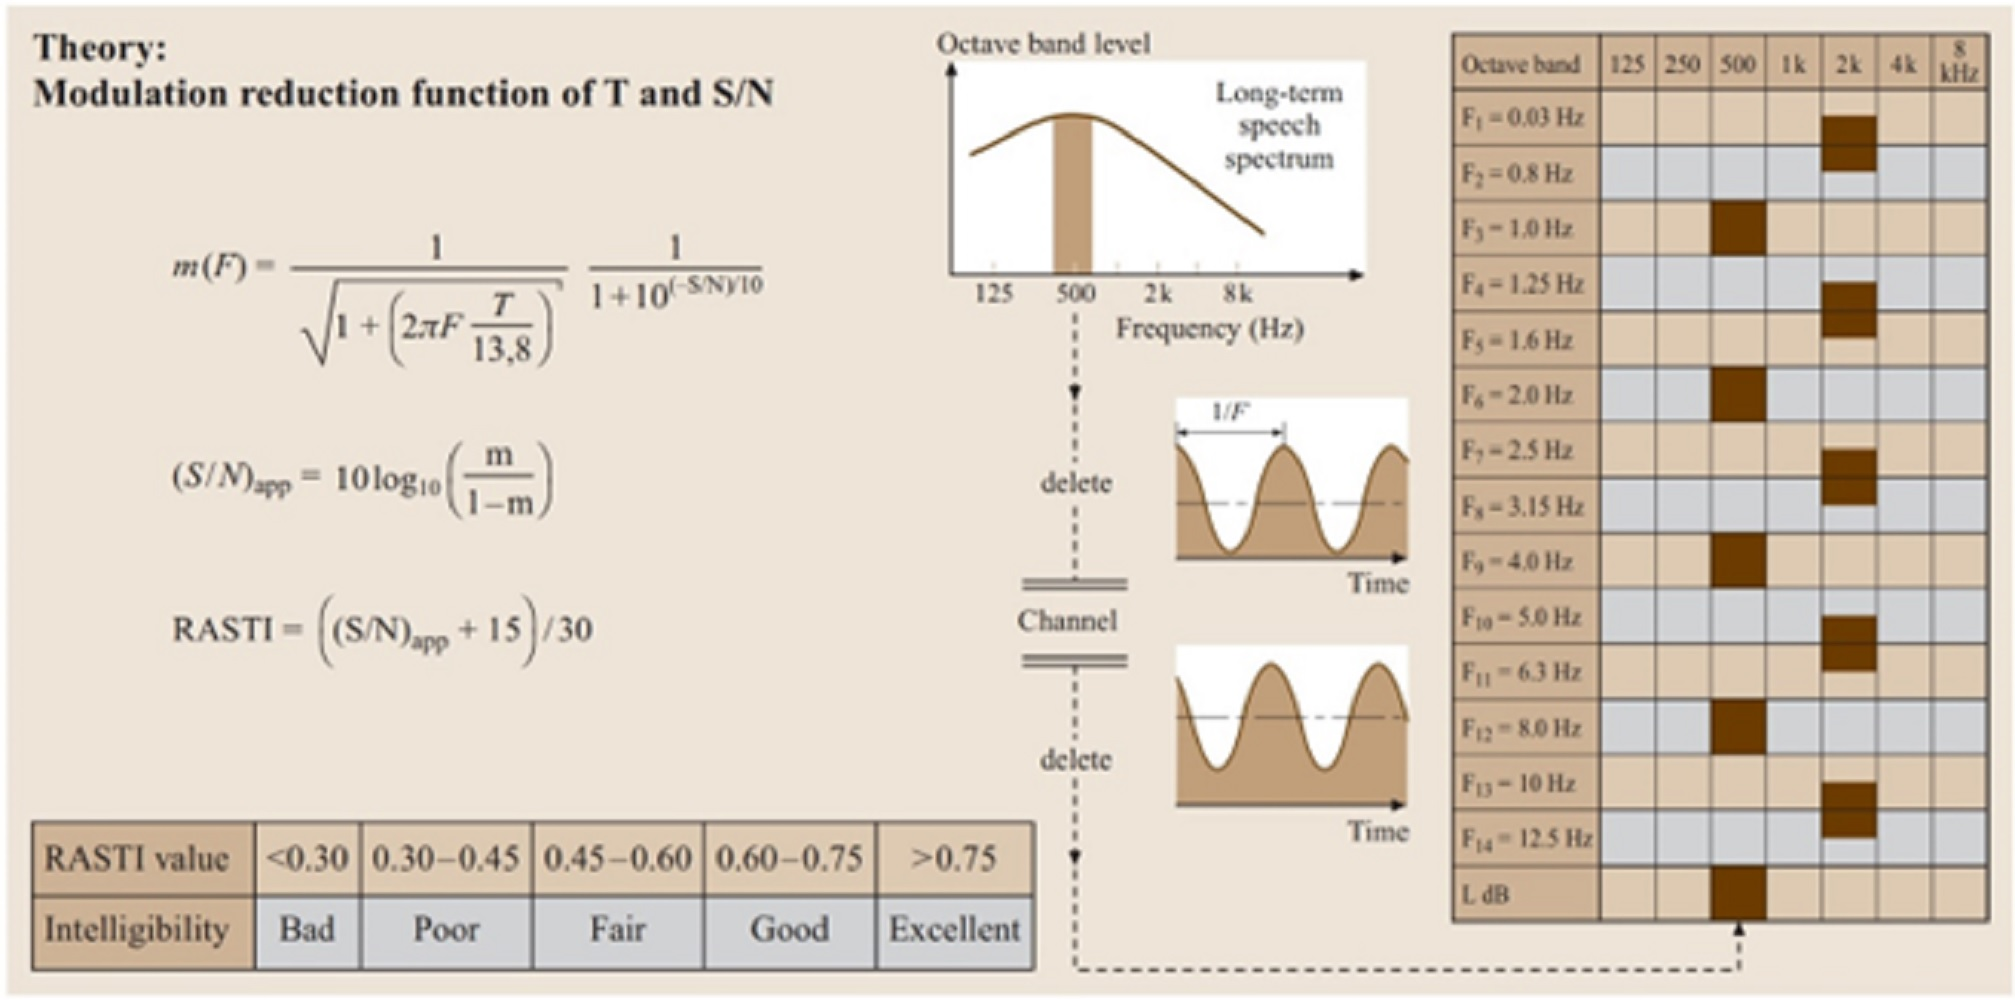
\includegraphics[width=0.9\textwidth]{imagenes/2.jpg}
    \caption{\footnotesize Ilustración de la teoría y el principio en la medición de STI o RASTI. La escala para la evolución de los valores RASTI se muestra en la parte inferior \cite{Rossing2007}.}
    \label{fig:IntelHabla}
\end{figure}
\FloatBarrier
